As described above, we plan a suite of comprehensive simulations of
XRBs and SNe Ia (both the sub-Ch and WDWD models) using our
codes \maestro\ and \castro.  All the problems we
describe are inherently three-dimensional, requiring large resources.
Our codes are running on titan today, and they perform and scale
well.  The starting point for all the simulations proposed are in
place.  We are ready to run.

The calculations we describe in further detail here are INCITE--class \MarginPar{needs updating}
for two reasons.  First, as is often the case in astrophysics, we can
never capture all the length-scales that come into play in these
stellar explosions, for example, the turbulent dissipation scale in
the convective regions is often quite below our grid resolution.  As a
result, we need to push to higher-and-higher resolution to assess
whether our results are converged.  This high resolution demands a lot
of computational resources---the type that only INCITE can provide.
Second, the temporal scales we need to model are equally impressive.
For the XRB simulations, we would like to model a second of evolution.
At our current resolution (6~cm), we would need over a million
timesteps (and that is with the large efficiency gain we get through
the low Mach model).  Since there is no parallel-in-time equivalent to
domain decomposition, we need to run a big problem for long amounts of
time on the machine---again, a feat only possible through INCITE.
Finally, we want to push the realism of the physics, in particular,
our reaction networks.  This will only be feasible by offloading some
of the reaction expense to the GPUs.

A key part of our collaboration is the emphasis on using GPUs
to accelerate the microphysics.  Both the Stony Brook and ORNL
groups have been working on this independently, and through this
proposal, we will unite our efforts to produce a set of community
GPU accelerated microphysics.  We will explore OpenACC, OpenMP 2.5,
and CUDA libraries to accomplish these goals, with an eye toward
summit.


The basic motivation for our science problems was given in the
previous section.  Here we begin by discussing the milestones we hope
to achieve in each year and then we give specific details about the
number and size of the simulations we plan to run.  We note that because
we have preliminary calculations of each of the problems we propose to
run, we can base our time requests on existing simulations from titan
(here Mh = mega-hours).  Also, there is a pattern to our milestones:
one milestone for each of the major topics per year (XRBs, sub-Ch,
WDWD, ...) with GPUs toward the end of the year, and the addition of 
new physics in year 2.  \MarginPar{read this}

\begin{tightitem}
\item {\bf Year 1: XX Mh total }
%
\begin{tightitem}
\item blah
\end{tightitem}
%
\item {\bf Year 2: XX~Mh total}
%
\begin{tightitem}
\item blah
\end{tightitem}
%
\end{tightitem}

\begin{figure}[t]
\centering
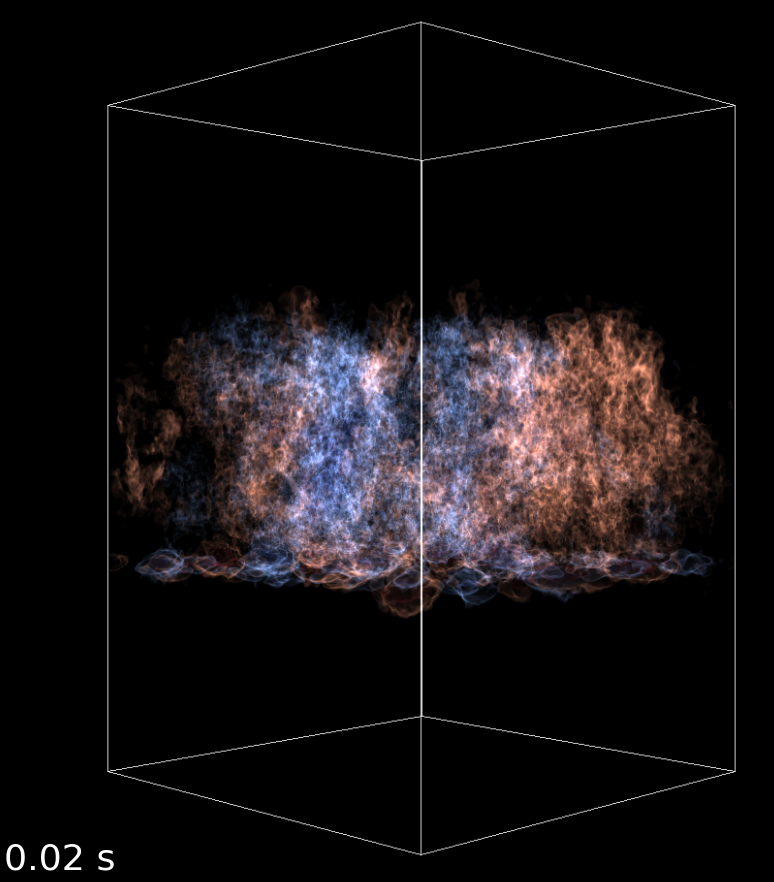
\includegraphics[width=0.28\linewidth]{xrb_compact}
\hspace{0.2em}
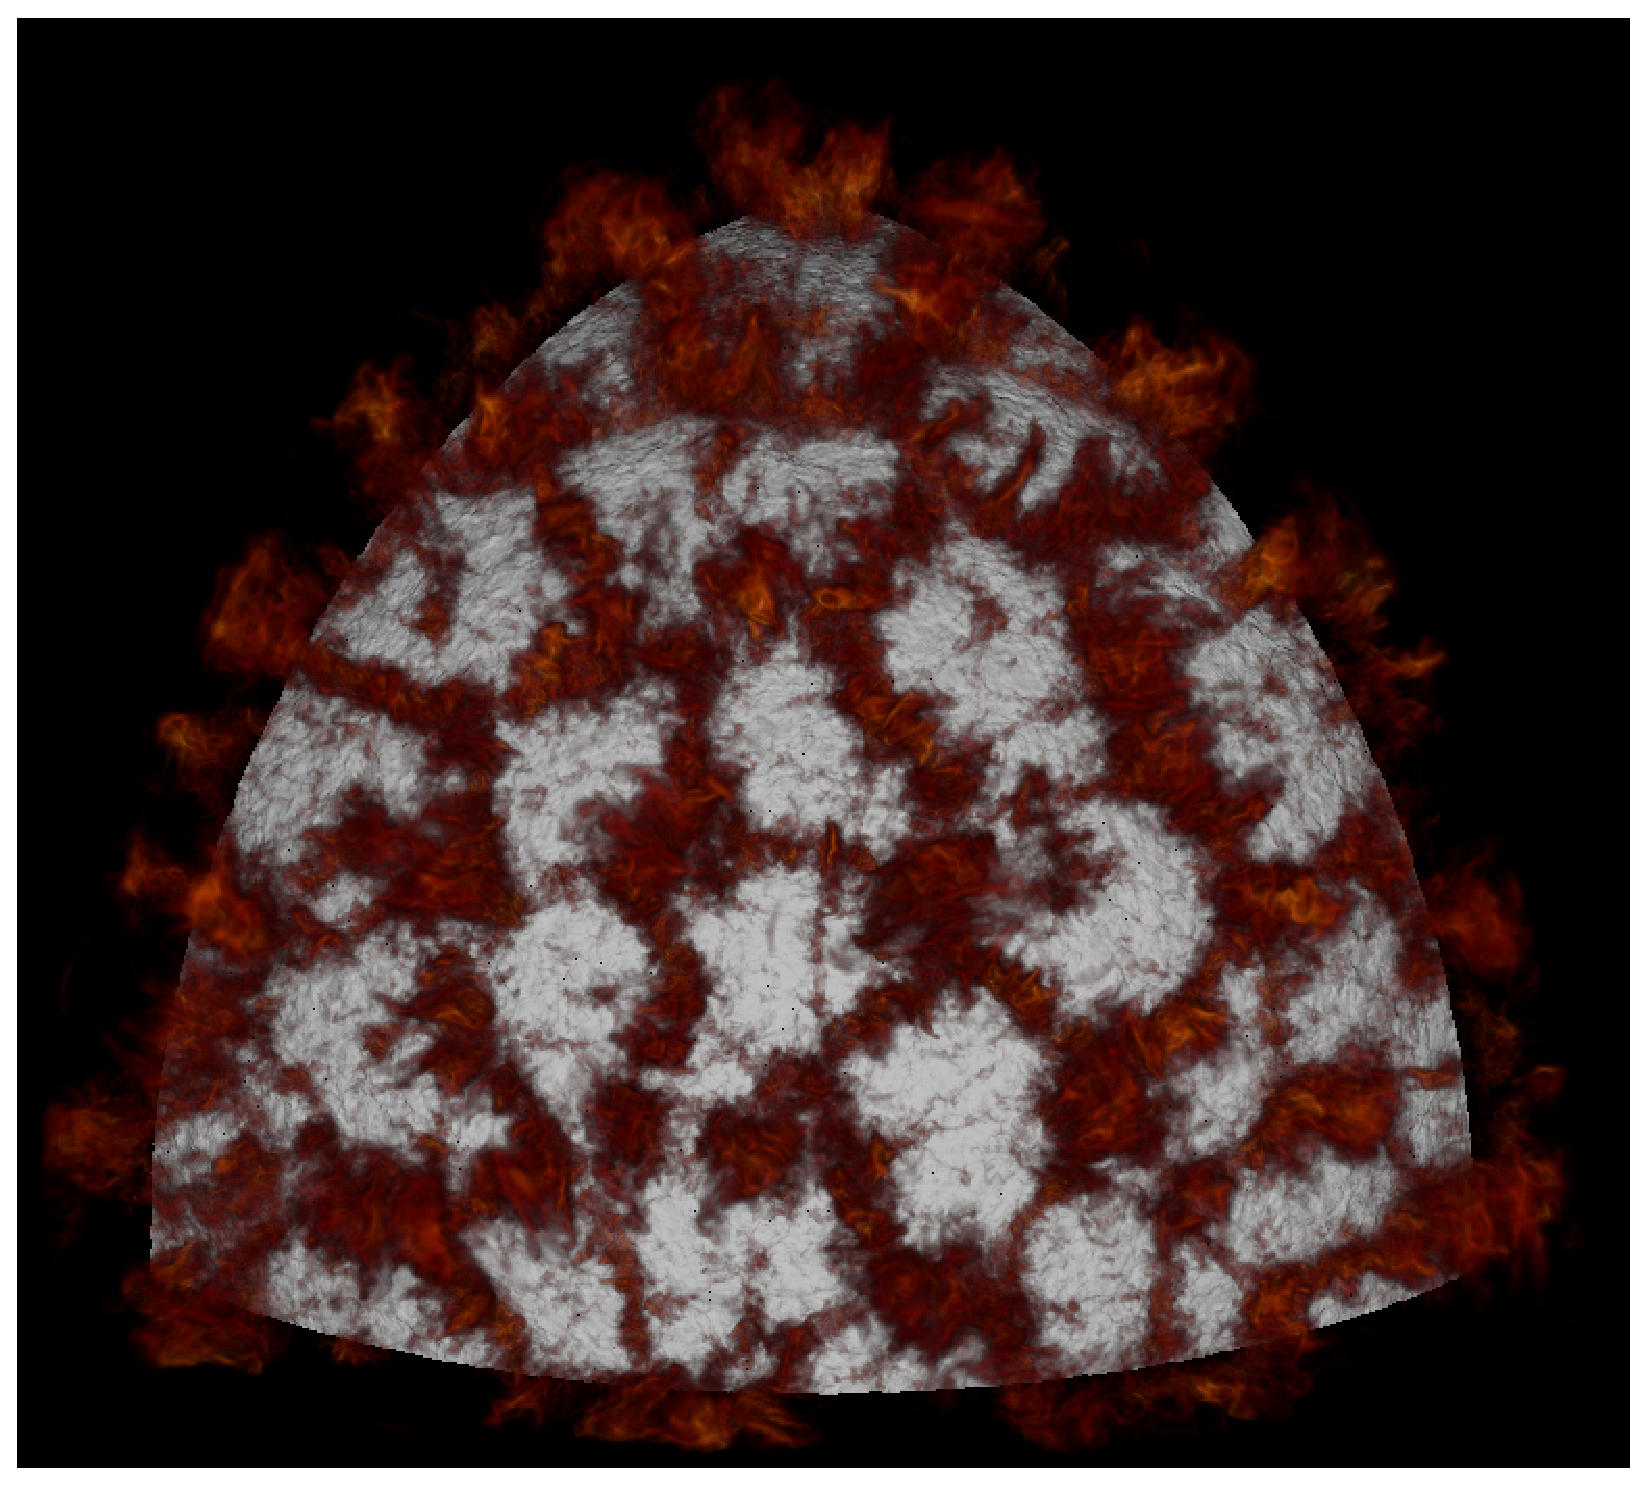
\includegraphics[width=0.28\linewidth]{ConvPlumes}
\hspace{0.2em}
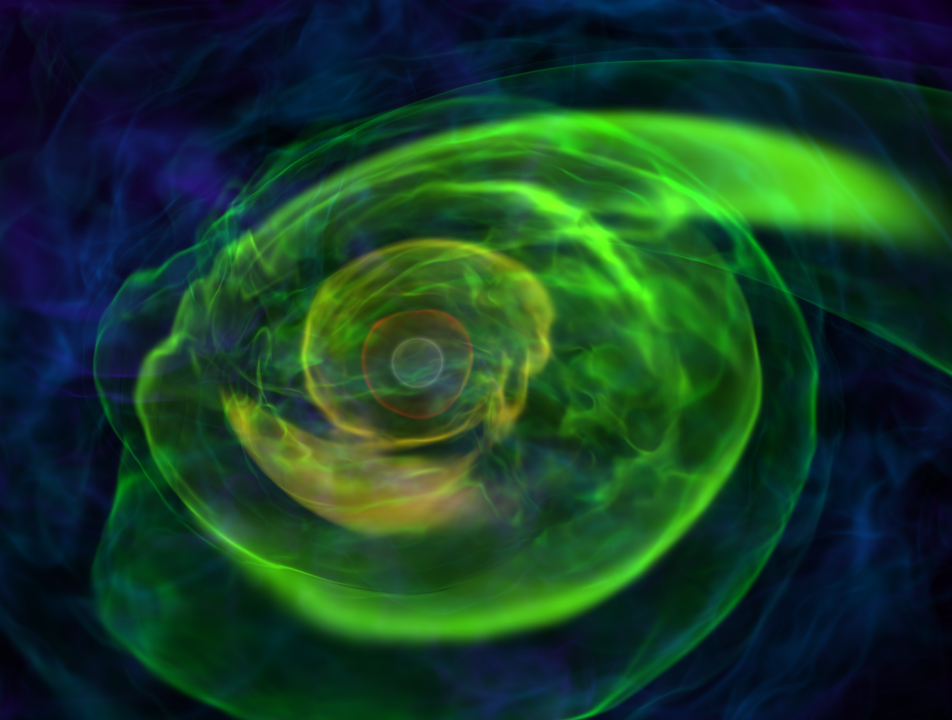
\includegraphics[width=0.4\linewidth]{wdmerger_08030_new.png}
\caption{\label{fig:current-runs} (top left) Vertical velocity showing the
  convective structure in a \maestro\ XRB calculation.  (top right)
  Convective plumes in a \maestro\ sub-Ch calculation.  (left)
  Snapshot of a \castro\ simulation of the merger of two white dwarfs,
  with 0.90 and 0.81 solar masses. The contours represent density
  levels. The star on the upper left is disrupting and accreting onto
  the other star.}
\end{figure}


{\bf SNe Ia simulations}:  


{\bf XRB simulations}:


{\bf CC SNe simulations}:


{\bf BWP simulations}:

{\bf Post processing and observables}:  
%
For the SNe Ia models that we bring to explosion, we will use the
\sedona\ radiation transfer code to produce synthetic observables
(lightcurves and spectra)---the \sedona\ author Dan Kasen is a Co-I on
this proposal.  This post processing was done with many of the explosion 
models in the current INCITE allocation and the pieces are in place for this
workflow. We do not expect \sedona\ to require a lot of compute
time for these models.


{\bf Exploratory simulations}:
%
We are
capable of modeling all phases of these explosive phenomena.  As a
result, when a new idea is promoted in the field, we will be in an
excellent position to explore it through detailed high-resolution
simulation.  We will keep pace with the field and propose some add-on
calculations in later year renewals.  One example already placed in
our milestones is the URCA calculation.



